\documentclass{beamer}
%
% Choose how your presentation looks.
%
% For more themes, color themes and font themes, see:
% http://deic.uab.es/~iblanes/beamer_gallery/index_by_theme.html
%
\mode<presentation>
{
  \usetheme{default}      % or try Darmstadt, Madrid, Warsaw, ...
  \usecolortheme{default} % or try albatross, beaver, crane, ...
  \usefonttheme{default}  % or try serif, structurebold, ...
  \setbeamertemplate{navigation symbols}{}
  \setbeamertemplate{caption}[numbered]
} 

\usepackage[english]{babel}
\usepackage[utf8]{inputenc}
\usepackage[T1]{fontenc}
\usepackage{hyperref}

\usepackage{minted}

\setminted[python]{ %
    linenos=false,             % Line numbers
    autogobble=true,          % Automatically remove common whitespace
    %bgcolor=dark-bg,
    frame=lines,
    framesep=2mm,
    fontsize=\footnotesize
}

\title[IRIS]{DIRAC install and basic usage}
\author{Iulia Cimpan}
\institute{UoM}
\date{7 Sept 2020}

\begin{document}

\begin{frame}
  \titlepage
\end{frame}

% Uncomment these lines for an automatically generated outline.
%\begin{frame}{Outline}
%  \tableofcontents
%\end{frame}



\begin{frame}{Introduction}
\begin{center}
\begin{itemize}
  \item get a grid certificate
\item join VO (Virtual Organisation)
\item add the certificate to your browser
\item install DIRAC UI
\item submit a job (python --version)
\item monitor a job
\item put data on the file catalog
\item submitting RASCIL job
\item get output data RASCIL job 
\item useful links
\footnote{What is IRIS: \url{https://www.iris.ac.uk/about-iris/} \newline
 Rich details GridPP:
\url{https://github.com/GridPP/user-guides} \newline
Getting Started:
\url{https://dirac.readthedocs.io/en/latest/UserGuide/GettingStarted/index.html}}
\end{itemize}
\end{center}
\end{frame}




\begin{frame}{Get A Grid Certificate}
\begin{center}
    \begin{itemize}
 \item a grid certificate is a .p12 file 
\item Using your browser of choice visit this page and select the Request New User Certificate option. This almost goes without saying, but make sure you supply a valid email address which you can access. You will also be asked to do things like supply a PIN and passwords that you will need later on, so make sure you write everything down!
\item You will need to select a Registration Authority (RA) as part of this process.You may also be asked to supply a letter of recommendation explaining why you need to use the grid and with whom you will be working.
\item Details at \footnote{grid certificate: \url{http://hep.ph.liv.ac.uk/~sjones/user-guides/getting-on-the-grid/grid-certificate.html}}
\end{itemize}
\end{center}
\end{frame}


\begin{frame}{Join a VO}
\begin{center}
    \begin{itemize}
 \item Your grid certificate identifies you to the grid as an individual user, but it's not enough on its own to allow you to use grid resources; you also need to join a Virtual Organisation (VO). 
\item Note: I have made my request to skatelescope.eu - see  \footnote{Approved Global VOs:
\url{https://www.gridpp.ac.uk/wiki/GridPP_approved_VOs}}
\item use the below link to register \footnote{register for a VO: \url{https://voms.gridpp.ac.uk:8443/voms/gridpp/register/start.action}}
\end{itemize}
\end{center}
\end{frame}

\begin{frame}{Add the Certificate to your Browser}
\begin{center}

\begin{itemize}
\item Now that you have the certificate and have joined to VO, you can add your certificate to your
browser and access DIRAC in browser \footnote{DIRAC in browser: \url{https://dirac.gridpp.ac.uk:8443/DIRAC/}}
\item More details about DIRAC at Guide to DIRAC \footnote{Guide to DIRAC: \url{https://www.gridpp.ac.uk/wiki/Quick_Guide_to_Dirac#Server_URL}}
\end{itemize}
\end{center}
\end{frame}


\begin{frame}{The Certificate in your Browser}
\begin{center}
  \begin{figure}
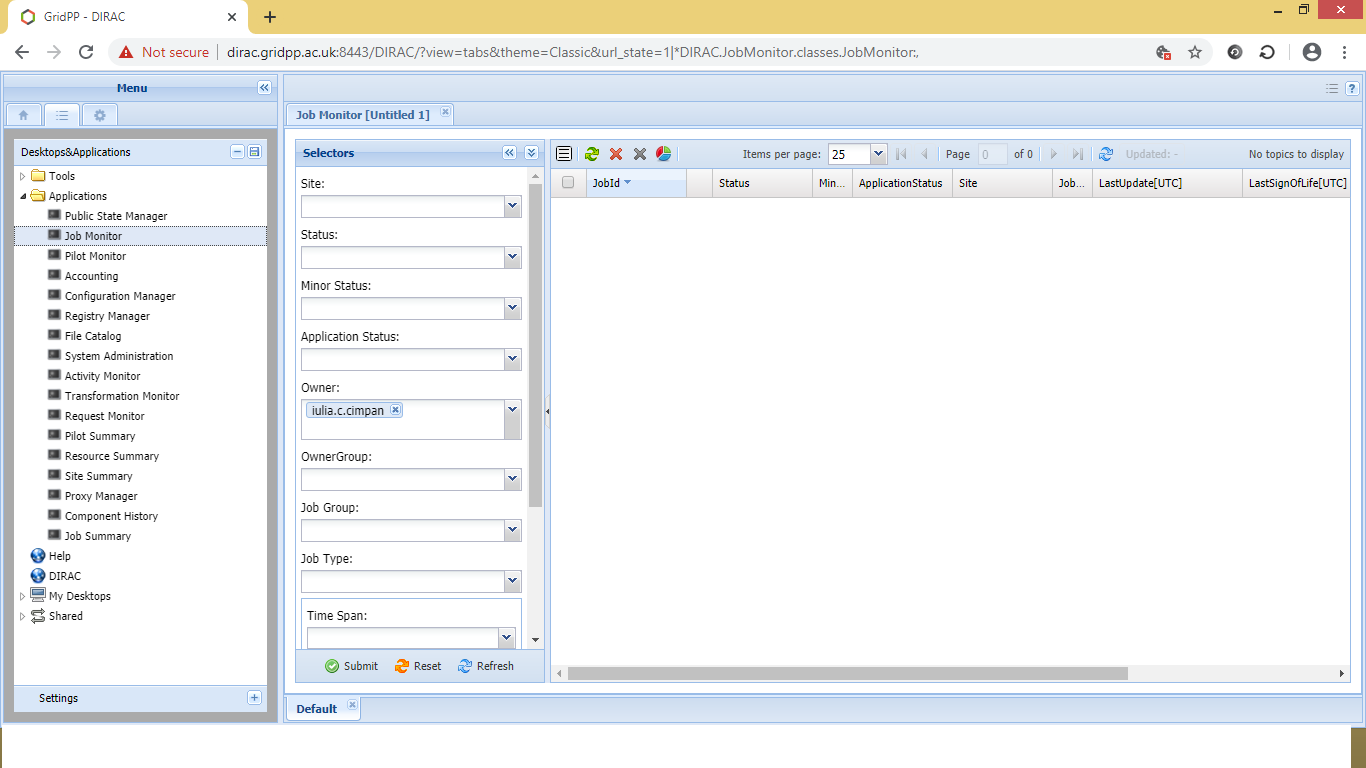
\includegraphics[scale=0.5]{DIRAC.png}
\caption{DIRAC}
\end{figure}
\end{center}
\end{frame}




\begin{frame}[fragile]
\frametitle{Before DIRAC install}
\textbf{}{Overview of directories on your server}
\begin{minted}{python}
/home/<your-user> - home directory

/raid/scratch/<your-user> - a working directory,
here DIRAC will be installed

FC:/............................ - belongs to IRIS, can
store large data. You need DIRAC installation to
be able to copy files to FC:/ (IRIS)

\end{minted}

\end{frame}


\begin{frame}[fragile]
\frametitle{ DIRAC install}
\textbf{Details at:} \footnote {Install Dirac: \url{https://github.com/as595/SKA-IRIS/blob/master/DIRACUI/InstallDirac.sh}}
\begin{minted}{python}
<your-user>@<your-server> /raid/scratch/<your-user> > mkdir dirac_ui
<your-user>@<your-server> /raid/scratch/<your-user> > cd dirac_ui/
<your-user>@<your-server> /raid/scratch/<your-user>/dirac_ui >
mkdir $HOME/.globus
<your-user>@<your-server> /raid/scratch/<your-user>/dirac_ui >ls
#make sure you have the cert in this folder dirac_ui, eg certBundle.p12
certBundle.p12 
\end{minted}
\end{frame}

\begin{frame}[fragile]
\frametitle{ DIRAC install}
\textbf{Details at:} \footnote{runMeForCertAndKey: \url{https://github.com/as595/SKA-IRIS/blob/master/DIRACUI/runMeForCertAndKey}}
\begin{minted}{python}
<your-user>@<your-server> /raid/scratch/<your-user>/dirac_ui > 
openssl pkcs12 -in certBundle.p12 -clcerts -nokeys -out 
$HOME/.globus/usercert.pem
Enter Import Password:
MAC verified OK
<your-user>@<your-server> /raid/scratch/<your-user>/dirac_ui > 
openssl pkcs12 -in certBundle.p12 -nocerts -out 
$HOME/.globus/userkey.pem
Enter Import Password:
MAC verified OK
Enter PEM pass phrase:
Verifying - Enter PEM pass phrase:
<your-user>@<your-server> /raid/scratch/<your-user>/dirac_ui > 
chmod 0400 $HOME/.globus/userkey.pem
\end{minted}
\end{frame}


\begin{frame}[fragile]
\frametitle{ DIRAC install}
\textbf{Details at:} \footnote {Install Dirac: \url{https://github.com/as595/SKA-IRIS/blob/master/DIRACUI/InstallDirac.sh}}
\begin{minted}{python}
<your-user>@<your-server> /raid/scratch/<your-user>/dirac_ui > 
wget -np -O dirac-install
https://raw.githubusercontent.com/DIRACGrid/DIRAC/integration/Core/sc
ripts/dirac-install.py
<your-user>@<your-server> /raid/scratch/<your-user>/dirac_ui > 
chmod u+x dirac-install
<your-user>@<your-server> /raid/scratch/<your-user>/dirac_ui > 
./dirac-install -r v6r22p6 -i 27 -g v14r1
\end{minted}
\end{frame}


\begin{frame}[fragile]
\frametitle{ DIRAC install}
\textbf{Details at:} \footnote {Install Dirac: \url{https://github.com/as595/SKA-IRIS/blob/master/DIRACUI/InstallDirac.sh}}
\begin{minted}{python}
<your-user>@<your-server> /raid/scratch/<your-user>/dirac_ui > source 
cshrc
<your-user>@<your-server> /raid/scratch/<your-user>/dirac_ui > 
dirac-proxy-init -x
Generating proxy...
Enter Certificate password:
<your-user>@<your-server> /raid/scratch/<your-user>/dirac_ui > 
dirac-configure -F -S GridPP -C
dips://dirac01.grid.hep.ph.ic.ac.uk:9135/Configuration/Server -I
<your-user>@<your-server> /raid/scratch/<your-user>/dirac_ui > 
dirac-proxy-init
-g skatelescope.eu_user -M 
#skatelescope.eu it is the VO I am assigned to
Generating proxy...
Enter Certificate password:
\end{minted}
\end{frame}


\begin{frame}[fragile]
\frametitle{ Submit a simple job}
\textbf{Details at:} \footnote {Simple Job: \url{https://dirac.readthedocs.io/en/latest/UserGuide/GettingStarted/UserJobs/CommandLine/index.html}}
\begin{minted}{python}
<your-user>@<your-server> /raid/scratch/<your-user>/dirac_ui > cat
simple.jdl
JobName = "InputAndOuputSandbox";
Executable = "pythonV.sh";
StdOutput = "StdOut";
StdError = "StdErr";
InputSandbox = {"pythonV.sh"};
OutputSandbox = {"StdOut","StdErr"};

<your-user>@<your-server> /raid/scratch/<your-user>/dirac_ui > 
cat pythonV.sh
#!/bin/bash
/usr/bin/python --version;

\end{minted}
\end{frame}


\begin{frame}[fragile]
\frametitle{ Monitor a simple job}
\textbf{Details at:} \footnote {Simple Job: \url{https://dirac.readthedocs.io/en/latest/UserGuide/GettingStarted/UserJobs/CommandLine/index.html}}
\begin{minted}{python}
<your-user>@<your-server> /raid/scratch/<your-user>/dirac_ui > 
dirac-wms-job-submit simple.jdl
JobID = 25104301

<your-user>@<your-server> /raid/scratch/<your-user>/dirac_ui > 
dirac-wms-job-status 25104301
JobID=25104301 Status=Done; MinorStatus=Execution Complete;
Site=LCG.UKI-NORTHGRID-MAN-HEP.uk;
\end{minted}
- The job execution can be seen also on
\href{https://dirac.gridpp.ac.uk:8443/DIRAC/}{DIRAC Web-link}
(see Applications/Job Monitor -> Owner (your name) -> submit)
\end{frame}


\begin{frame}[fragile]
\frametitle{ Put RASCIL.img in a file catalog}
\textbf{Details at:} \footnote {File Catalog: \url{https://dirac.readthedocs.io/en/latest/UserGuide/CommandReference/DataManagement/index.html}}
\begin{minted}{python}
<your-user>@<your-server> /raid/scratch/<your-user>/dirac_ui > 
dirac-dms-add-file LFN:/skatelescope.eu/user/<first letter of your
user>/<your-user>/rascil/RASCIL.img RASCIL.img UKI-NORTHGRID-
MAN-HEP-disk
# UKI-NORTHGRID-MAN-HEP-disk - SE: DIRAC Storage Element

Then you will find the file RASCIL.img under: 
FC:/skatelescope.eu/user/<first letter of your
user>/<your-user>/rascil/RASCIL.img
\end{minted}
\end{frame}



\begin{frame}[fragile]
\frametitle{Submitting RASCIL job}
\textbf{Details at:} \footnote {Simple Job: \url{https://dirac.readthedocs.io/en/latest/UserGuide/GettingStarted/UserJobs/CommandLine/index.html}}
\begin{minted}{python}
cat simpleR1.jdl
JobName    = "InputAndOuputSandbox";
Executable = "testR1.sh";
StdOutput = "StdOut";
StdError = "StdErr";
InputSandbox = {"testR1.sh"};
InputData = {"LFN:/skatelescope.eu/user/c/cimpan/rascil/
RASCIL-full1.img"};
OutputSandbox = {"StdOut","StdErr","imaging_dirty.fits",
"imaging_psf.fits","imaging_restored.fits"};
OutputSE ="UKI-NORTHGRID-MAN-HEP-disk";
Site = "LCG.UKI-NORTHGRID-MAN-HEP.uk";

 cat testR1.sh
#!/bin/bash
singularity exec --cleanenv -H $PWD:/srv --pwd /srv -C 
RASCIL-full1.img python3 /rascil/examples/scripts/imaging.py;


\end{minted}
\end{frame}


\begin{frame}[fragile]
\frametitle{Managing RASCIL job}
\textbf{Details at:} \footnote {Simple Job: \url{https://dirac.readthedocs.io/en/latest/UserGuide/GettingStarted/UserJobs/CommandLine/index.html}}
\begin{minted}{python}
$ dirac-wms-job-submit simpleR1.jdl
JobID = 25260750

$ dirac-wms-job-status  25260750
JobID=25260750 Status=Running; MinorStatus=Input Data Resolution; 
Site=LCG.UKI-NORTHGRID-MAN-HEP.uk;

$ dirac-wms-job-status  25260750
JobID=25260750 Status=Done; MinorStatus=Execution Complete; 
Site=LCG.UKI-NORTHGRID-MAN-HEP.uk;
\end{minted}
\end{frame}


\begin{frame}[fragile]
\frametitle{Get Output Data RASCIL job}
\textbf{Details at:} \footnote {Simple Job: \url{https://dirac.readthedocs.io/en/latest/UserGuide/GettingStarted/UserJobs/CommandLine/index.html}}
\begin{minted}{python}
Note: the RASCIL job has 3 image outputs, so we specify them in 
OutputSandbox and we take the data locally using command

$ dirac-wms-job-get-output  25260750
Job output sandbox retrieved in 
/raid/scratch/<your-user>/dirac_ui/tests/rascilTests/25260750/
$ cd 25260750
$ ls
imaging_dirty.fits  imaging_psf.fits  imaging_restored.fits  StdOut
$ cat StdOut   #or StdErr
\end{minted}
\end{frame}

\begin{frame}{Useful Links}
\begin{center}
    \begin{itemize}
 \item What is IRIS: \href{https://www.iris.ac.uk/about-iris/}{ link} 

\item Rich details GridPP user-guide at:    \href{https://github.com/GridPP/user-guides}{link}

\item Getting on the grid: \href{https://github.com/gridpp/user-guides/tree/master/getting-on-the-grid}{link}

\item Useful command DIRAC UI install: \href{https://github.com/as595/SKA-IRIS/tree/master/DIRACUI}{link}

\item Getting started: \href{https://dirac.readthedocs.io/en/latest/UserGuide/GettingStarted/index.html}{link}

\item Getting started User Jobs:
\href{https://dirac.readthedocs.io/en/latest/UserGuide/GettingStarted/UserJobs/index.html}{link}

\item Getting started Data Management:
\href{https://dirac.readthedocs.io/en/latest/UserGuide/CommandReference/DataManagement/index.html}{link}

\item Getting started Command Line:
\href{https://dirac.readthedocs.io/en/latest/UserGuide/GettingStarted/UserJobs/CommandLine/index.html}{link}

\end{itemize}
\end{center}
\end{frame}


\end{document}

